\documentclass[nojss]{jss}\usepackage[]{graphicx}\usepackage[]{color}
%% maxwidth is the original width if it is less than linewidth
%% otherwise use linewidth (to make sure the graphics do not exceed the margin)
\makeatletter
\def\maxwidth{ %
  \ifdim\Gin@nat@width>\linewidth
    \linewidth
  \else
    \Gin@nat@width
  \fi
}
\makeatother

\usepackage{Sweave}



%\usepackage{setspace}
% \usepackage[sc]{mathpazo}
\usepackage{amsmath}
% %\usepackage{geometry} 
% %\geometry{verbose, tmargin = 1.25cm, bmargin = 1.25cm, lmargin = 1.25cm, rmargin = 1.25cm}
% \setcounter{secnumdepth}{2}
% \setcounter{tocdepth}{2}
\usepackage{longtable}
\usepackage{colortbl, xcolor}
\usepackage{booktabs}

%%%%%%%%%%%%%%%%%%%%%%%%%%%%%%
%% declarations for jss.cls %%
%%%%%%%%%%%%%%%%%%%%%%%%%%%%%%
%\VignetteEngine{knitr::knitr}
%\VignetteIndexEntry{survivalRandomForest}
%\VignetteIndexEntry{Random Forests for Survival ggRandomForests packages}                     
%\VignetteKeywords{random forest, survival, VIMP, minimal depth}                                  
%\VignetteDepends{ggRandomForests}                   
%\VignettePackage{ggRandomForests} 

%% almost as usual
\author{John Ehrlinger 
\and Eugene H. Blackstone\\Cleveland Clinic}

\title{\pkg{ggRandomForests}: Survival with Random Forests}

%% for pretty printing and a nice hypersummary also set:
\Plainauthor{Ehrlinger et.\ al.} %% comma-separated
\Plaintitle{ggRandomForests: Random Forests for Survival} %% without formatting
\Shorttitle{Random Forests for Survival}

%% an abstract and keywords
\Abstract{ 
Random Forests~\citep{Breiman:2001} (RF) are a fully non-parametric statistical method requiring no distributional assumptions on covariate relation to the response. RF are a robust, nonlinear technique that optimizes predictive accuracy by fitting an ensemble of trees to stabilize model estimates. Random Forests for survival~\citep{Ishwaran:2007a, Ishwaran:2008} (RF-S) are an extension of Breiman's RF techniques to survival settings, allowing efficient non-parametric analysis of time to event data. The \pkg{randomForestSRC} package~\citep{Ishwaran:RFSRC:2014} is a unified treatment of Breiman's random forests for survival, regression and classification problems.

Predictive accuracy make RF an attractive alternative to parametric models, though complexity and interpretability of the forest hinder wider application of the method. We introduce the \pkg{ggRandomForests} package, tools for creating and plotting data structures to visually understand random forest models grown in \proglang{R} with the \pkg{randomForestSRC} package. The \pkg{ggRandomForests} package is structured to extract intermediate data objects from \pkg{randomForestSRC} objects and generate figures using the \pkg{ggplot2}~\citep{Wickham:2009} graphics package.

This document is formatted as a tutorial for using the \pkg{randomForestSRC} for building random forests for survival and \pkg{ggRandomForests} package for investigating how the forest is constructed. This tutorial uses the Primary Biliary Cirrhosis (PBC) Data from the Mayo Clinic~\citep{fleming:1991} available in the \pkg{randomForestSRC} package. We use Variable Importance measure (VIMP)~\citep{Breiman:2001} as well as Minimal Depth~\citep{Ishwaran:2010}, a property derived from the construction of each tree within the forest, to assess the impact of variables on forest prediction. We will also demonstrate the use of variable dependence plots~\citep{Friedman:2000} to aid interpretation RF results in different response settings. We also will investigate interactions between covariates to demonstrate the strength of the Random Forest method in survival settings.
}
\Keywords{random forest, survival, VIMP, minimal depth, \proglang{R}, \pkg{randomForestSRC}}
\Plainkeywords{random forest, survival, VIMP, minimal depth, R, randomForestSRC}
%% at least one keyword must be supplied

%% publication information
%% NOTE: Typically, this can be left commented and will be filled out by the technical editor
%% \Volume{13}
%% \Issue{9}
%% \Month{September}
%% \Year{2004}
%% \Submitdate{2004-09-29}
%% \Acceptdate{2004-09-29}

%% The address of (at least) one author should be given
%% in the following format:
\Address{
John Ehrlinger\\
Quantitative Health Sciences\\
Lerner Research Institute\\
Cleveland Clinic\\
9500 Euclid Ave\\
Cleveland, Ohio 44195\\
% Telephone: + 41/0/44634-4643 \\
% Fax: + 41/0/44634-4386 \\
E-mail: \email{john.ehrlinger@gmail.com}\\
URL: \url{http://www.lerner.ccf.org/qhs/people/ehrlinj/}
}

%% It is also possible to add a telephone and fax number
%% before the e-mail in the following format:
%% Telephone: + 43/1/31336-5053
%% Fax: + 43/1/31336-734

%% for those who use Sweave please include the following line (with % symbols):
%% need no \usepackage{Sweave.sty}

%% end of declarations %%%%%%%%%%%%%%%%%%%%%%%%%%%%%%%%%%%%%%%%%%%%%%%



\IfFileExists{upquote.sty}{\usepackage{upquote}}{}
\begin{document}
% -----------------------------------------------------
\section{About this document}
% -----------------------------------------------------
This document is an introduction to the \pkg{ggRandomForests} \proglang{R} package. The aim of this introduction is to provide a detailed user guide to \pkg{ggRandomForests} as well as provide a tutorial to building a Random Forest Survival model with the \pkg{randomForestSRC} package. Our attempt is to build simple, reproducible worked examples with the Primary Biliary Cirrhosis (PBC) Data from the Mayo Clinic.

This document is available as a vignette within \pkg{ggRandomForests} package. The latest version is available from the Comprehensive \proglang{R} Archive Network via \url{http://CRAN.R-project.org/package = ggRandomForests}.

% -----------------------------------------------------
\section{Introduction} \label{S:introduction}
% -----------------------------------------------------

Random Forests~\citep{Breiman:2001} (RF) are a robust, non-parametric statistical method that optimizes predictive accuracy by averaging an ensemble of tree models. Random Forests are not parsimonious, utilizing all provided variables in predicting the specified outcome. It does not require prior knowledge of the parametric relation of variables (linearity or non-linearity) to the response, or of interactions between variables. RF chooses the most important variables by assessing variable impact on the predictive ability of the forest of trees.

A Random Forest is built up by bagging~\citep{Breiman:1996} a collection of classification and regression trees~\citep{cart:1984} (CART). The method uses a set of $B$ bootstrap~\citep{bootstrap:1994} samples, growing a set of independent tree models on each sub-sample of the population. Trees are grown by recursively partitioning the population based on optimization of a split rule over the $p$ dimensional covariate space. At each split, a subset of $m \le p$ candidate variables are chosen for the splitting. Each node is split into two daughter nodes by maximizing the separation of observations according the split rule. In regression trees, node impurity is measured by mean squared error, whereas in classification problems, the Gini index is used~\citep{Friedman:2000}. Each subsequent daughter node is then split until the process reaches the stopping criteria of either node purity or node member size defining the set of terminal (unsplit) nodes for the tree. Random Forests sort each observation into one unique terminal node per tree. The Random Forest estimate for each observation is calculated by aggregation, averaging (regression) or votes (classification), the terminal node results across the collection of $B$ trees. 

One advantage of Random Forests is a built in generalization error estimate. Each bootstrap sample selects approximately $63.2\%$ of the population on average. The remaining $36.8\%$ of observations, the Out-of-Bag~\citep{BreimanOOB:1996e} (OOB) sample, can be used as a hold out test set for each tree. An OOB prediction error estimate can be calculated for each observation by predicting the response over the set of trees which were NOT trained with that particular observation. Out-of-Bag prediction error estimates have been shown to be nearly identical to $n$--fold cross validation estimates~\citep{StatisticalLearning:2009}. This feature of Random Forests allows us to obtain both model fit and validation in one pass of the algorithm.

\subsection{Random Forests for Survival}\label{S:rfs}
Random Forests for survival~\citep{Ishwaran:2007, Ishwaran:2008} (RF-S) are an extension of~\cite{Breiman:2001} Random Forests for right censored time to event data. A forest of survival trees is grown using a log-rank splitting rule to select the optimal candidate variables. Survival estimate for each observation are constructed with a Kaplan--Meier (KM) estimator within each terminal node, at each event time. 

Random Forests for survival adaptively discover nonlinear effects and interactions and are fully nonparametric. Averaging over trees, with randomizing while growing a tree, enables RF-S to approximate complex survival functions, including non-proportional hazards, while maintaining low prediction error. \cite{Ishwaran:2010a} showed that RF-S is uniformly consistent and that survival forests have a uniform approximating property in finite-sample settings, a property not possessed by individual survival trees.

\subsection{ggRandomForests}
The \pkg{randomForestSRC} package is a mature analysis and research random forest implementation under rapid development. The package includes diagnostic and post processing functions for analysis and visualizations of randomForest model properties. However, in our research we frequently found it difficult to manipulate the standard figures directly produced with the \pkg{randomForestSRC} package. 

In order to simplify these manipulations, we developed the \pkg{ggRandomForests} package. We attempted to follow two design principles in this development:
\begin{itemize}
\item Model/View separation: The package originally designed to generating \pkg{ggplot2}~\cite{Wickham:2009} figures for random forest objects. However, some users would prefer to use other graphing methods within \proglang{R} or outside of it. To help users, we separate the data generation and the figure generation into two separate operations. 

\item Modular: We strive to create a modular design by following the \emph{do one thing well} philosphy. Each function operates on one \pkg{randomForestSRC} object to create only one data object or figure type.
\end{itemize}

To demonstrate using the \pkg{ggRandomForests} package, we organize this document as follows. In Section~\ref{S:rfsrcGrow} we outline growing a random forest for each of the classification, regression and survival settings with the \pkg{randomForestSRC} package. We use the \pkg{ggRandomForests} package to begin exploring random forest convergence and prediction. In Section~\ref{S:variableIdentification} we discuss how variables contribute to the random forest prediction using the Variable Importance (VIMP) and Minimal Depth measures.

Once we have an idea which variables are most informative in minimizing forest prediction error, we turn our focus to how the variables are related to the forest prediction. Because Random Forests are non-linear and non-parametric predictors, we can use variable dependence (Section~\ref{S:variableDependence}) to examine where each observation contributes to model prediction as a function of specific covariate values. Partial dependence (Section~\ref{S:partialDependence}) gives us a risk adjust view of the predictor dependence on a variable. We then find two way interactions using minimal depth in Section~\ref{S:interactions} and use conditional plots in Section~\ref{S:coplots} to look variable interactions in an intuitive manner.

\section{Data Summary: Primary Biliary Cirrhosis (PBC) Data}

Data from the Mayo Clinic trial in primary biliary cirrhosis (PBC) of the liver conducted between 1974 and 1984. A total of 424 PBC patients, referred to Mayo Clinic during that ten-year interval, met eligibility criteria for the randomized placebo controlled trial of the drug D-penicillamine. The first 312 cases in the data set participated in the randomized trial and contain largely complete data~\citep{fleming:1991}.



% latex table generated in R 3.1.2 by xtable 1.7-4 package
% Wed Dec 24 14:07:51 2014
\begin{table}[ht]
\centering
{\footnotesize
\begin{tabular}{rll}
  \toprule
 & label & type \\ 
  \midrule
status & censoring indicator & logical \\ 
   \rowcolor[gray]{0.95}treatment & Treament & factor \\ 
  age & age in years & numeric \\ 
   \rowcolor[gray]{0.95}sex & Female & logical \\ 
  ascites & Asictes & logical \\ 
   \rowcolor[gray]{0.95}hepatom & Hepatomegaly & logical \\ 
  spiders & Spiders & logical \\ 
   \rowcolor[gray]{0.95}edema & Edema & factor \\ 
  bili & serum bilirubin (mg/dl) & numeric \\ 
   \rowcolor[gray]{0.95}chol & serum cholesterol (mg/dl) & integer \\ 
  albumin & albumin (gm/dl) & numeric \\ 
   \rowcolor[gray]{0.95}copper & urine copper (ug/day) & integer \\ 
  alk & alkaline phosphatase (U/liter) & numeric \\ 
   \rowcolor[gray]{0.95}sgot & SGOT (U/ml) & numeric \\ 
  trig & triglicerides (mg/dl) & integer \\ 
   \rowcolor[gray]{0.95}platelet & platelets per cubic ml/1000 & integer \\ 
  prothrombin & prothrombin time (sec) & numeric \\ 
   \rowcolor[gray]{0.95}stage & histologic stage & factor \\ 
  years & survival time (years) & numeric \\ 
   \rowcolor[gray]{0.95} \bottomrule
\end{tabular}
}
\caption{PBC Data field descriptions} 
\label{T:dataLabs}
\end{table}



\begin{Schunk}
\begin{Sinput}
R> gg_dta <- gg_survival(interval="years",censor="status", 
+                       strat="treatment", data=pbc[-which(is.na(pbc$treatment)),] )
R> plot(gg_dta, se=.95) +
+   labs(y="Survival Probability", x="Observation Time (years)", 
+        color="Treatment", fill="Treatment")+
+   theme(legend.position=c(.2,.2))
\end{Sinput}
\begin{figure}[!htpb]

{\centering \includegraphics[width=\maxwidth]{figure/rfs-gg_survival-1} 

}

\caption[Kaplan-Meier pbc data survival estimates comparing the treatment with placebo]{Kaplan-Meier pbc data survival estimates comparing the treatment with placebo. Mean survival with shaded 95\% condfidence band.\label{fig:gg_survival}}
\end{figure}
\end{Schunk}

\begin{Schunk}
\begin{Sinput}
R> pbc.alt <- pbc[-which(is.na(pbc$treatment)),]
R> pbc.alt$bili_grp <- cut(pbc.alt$bili, 
+                         breaks=c(0,.8,1.3,3.4,max(pbc.alt$bili)))
R> 
R> gg_dta <- gg_survival(interval="years",censor="status", 
+                       strat="bili_grp", data=pbc.alt )
R> 
R> plot(gg_dta, error="none") +
+   labs(y="Survival Probability", 
+        x="Observation Time (years)", 
+        color="Bilirubin")
\end{Sinput}
\begin{figure}[!htpb]

{\centering 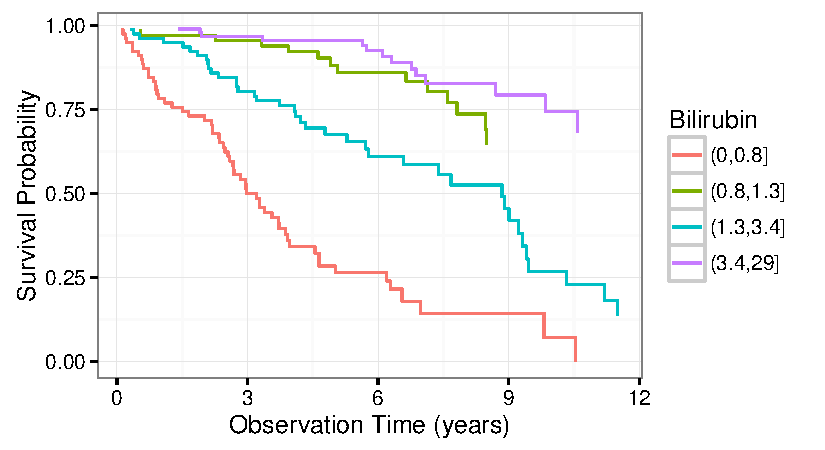
\includegraphics[width=\maxwidth]{figure/rfs-gg_survival-bili-1} 

}

\caption[Kaplan-Meier pbc data survival estimates comparing Bilirubin measures]{Kaplan-Meier pbc data survival estimates comparing Bilirubin measures.\label{fig:gg_survival-bili}}
\end{figure}
\end{Schunk}

% latex table generated in R 3.1.2 by xtable 1.7-4 package
% Wed Dec 24 14:07:51 2014
\begin{table}[ht]
\centering
{\footnotesize
\begin{tabular}{rrrr}
  \toprule
 & Coef. & Std. Err. & Z stat. \\ 
  \midrule
Age & 0.0333 & 0.0087 & 3.8400 \\ 
   \rowcolor[gray]{0.95}log(Albumin) & -3.0553 & 0.7241 & -4.2200 \\ 
  log(Bilirubin & 0.8792 & 0.0987 & 8.9000 \\ 
   \rowcolor[gray]{0.95}Edema & 0.7847 & 0.2991 & 2.6200 \\ 
  log(Prothrombin Time) & 3.0157 & 1.0238 & 2.9500 \\ 
   \rowcolor[gray]{0.95} \bottomrule
\end{tabular}
}
\caption{Regression model with log transformations of continuous variables, 312 randomized cases with PBC.} 
\label{T:FHmodel}
\end{table}

\section{Growing the Random Forest}

\begin{Schunk}
\begin{Sinput}
R> rfsrc_pbc <- rfsrc(Surv(years, status) ~ ., data = pbc, 
+                    nsplit = 10, 
+                    na.action = "na.impute")
R> rfsrc_pbc
\end{Sinput}
\end{Schunk}

\begin{Schunk}
\begin{Soutput}
                         Sample size: 312
                    Number of deaths: 125
                    Was data imputed: yes
                     Number of trees: 1000
          Minimum terminal node size: 3
       Average no. of terminal nodes: 59.902
No. of variables tried at each split: 5
              Total no. of variables: 17
                            Analysis: RSF
                              Family: surv
                      Splitting rule: logrank *random*
       Number of random split points: 10
                          Error rate: 16.01%
\end{Soutput}
\end{Schunk}

\begin{Schunk}
\begin{figure}[!htpb]

{\centering 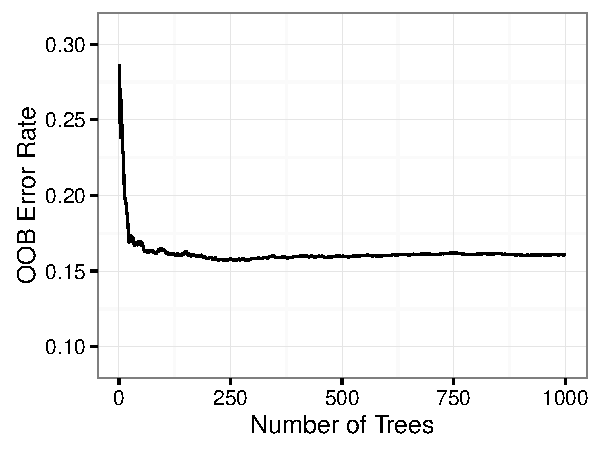
\includegraphics[width=\maxwidth]{figure/rfs-errorPlot-1} 

}

\caption[Random forest prediction error estimates as a function of the number of trees in the forest]{Random forest prediction error estimates as a function of the number of trees in the forest.\label{fig:errorPlot}}
\end{figure}
\end{Schunk}

Figure~\ref{fig:rfsrc-plot} shows the predicted survival from an RF-S model, where censored device prediction is colored in blue, and devices experiencing an event are colored in red. 
\begin{Schunk}
\begin{figure}[!htpb]

{\centering 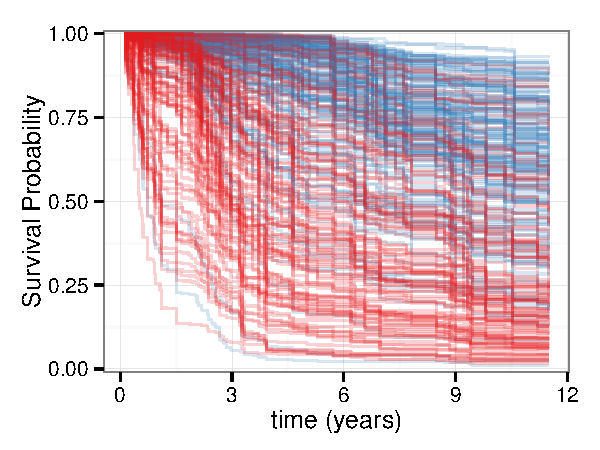
\includegraphics[width=\maxwidth]{figure/rfs-rfsrc-plot-1} 

}

\caption[Random forest predicted survival]{Random forest predicted survival. Blue lines correspond to censored observations, red lines correspond to patients who experienced the event (death).\label{fig:rfsrc-plot}}
\end{figure}
\end{Schunk}

\begin{Schunk}
\begin{figure}[!htpb]

{\centering \includegraphics[width=\maxwidth]{figure/rfs-rfsrc-plot-split-1} 

}

\caption[Random forest predicted survival]{Random forest predicted survival. Split on death event, black loess curve indicates the mean survival estimate within each group.\label{fig:rfsrc-plot-split}}
\end{figure}
\end{Schunk}

\begin{Schunk}
\begin{figure}[!htpb]

{\centering 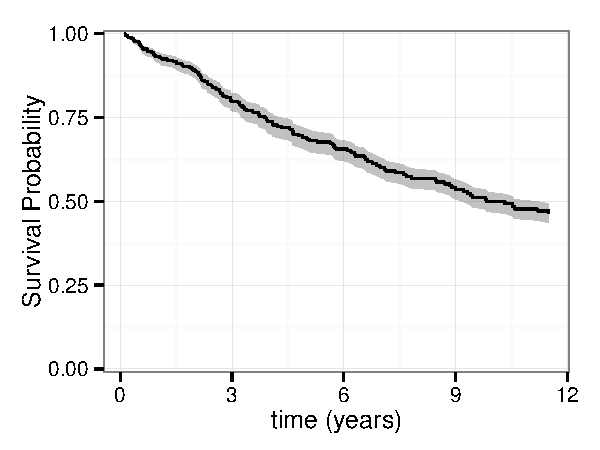
\includegraphics[width=\maxwidth]{figure/rfs-rfsrc-mean-1} 

}

\caption[Mean value random forest predicted survival with shaded 95\% confidence band]{Mean value random forest predicted survival with shaded 95\% confidence band.\label{fig:rfsrc-mean}}
\end{figure}
\end{Schunk}

\begin{Schunk}
\begin{figure}[!htpb]

{\centering 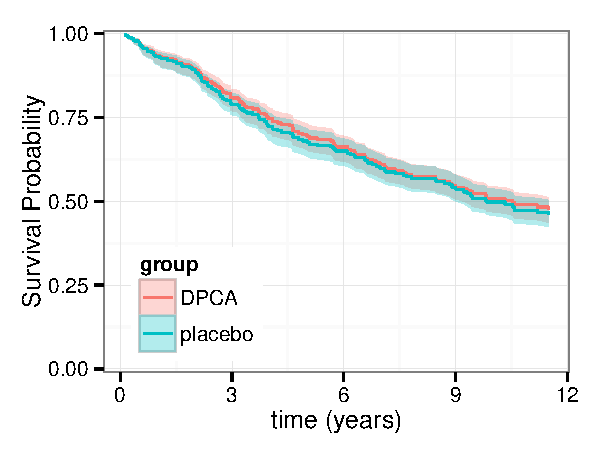
\includegraphics[width=\maxwidth]{figure/rfs-rfsrc-mean2-1} 

}

\caption[Mean value random forest predicted survival with shaded 95\% confidence band]{Mean value random forest predicted survival with shaded 95\% confidence band.\label{fig:rfsrc-mean2}}
\end{figure}
\end{Schunk}
\subsection{Forest Imputation for missing values}\label{S:imputation}

The randomForests package~\citep{liaw:2002} include a forest imputation method within the randomForest package. 

We impute missing data (both x and y-variables) using a modification of the missing data algorithm of~\cite{Ishwaran:2008}. Prior to splitting a node, missing data for a variable is imputed by randomly drawing values from non-missing in-bag data. The purpose of the imputed data is to make it possible to assign cases to daughter nodes in the event the node is split on a variable with missing data. Imputed data is however not used to calculate the split-statistic which uses non-missing data only. Following a node split, imputed data are reset to missing and the process is repeated until terminal nodes are reached. Missing data is then imputed using OOB non-missing terminal node data. For integer valued variables and censoring indicators, imputation uses a maximal class rule, whereas continuous variables and survival time use a mean rule.

The proximity matrix from the randomForest is used to update the imputation of the NAs. For continuous predictors, the imputed value is the weighted average of the non-missing obervations, where the weights are the proximities. For categorical predictors, the imputed value is the category with the largest average proximity. This process is iterated iter times.

Regardless of what method is used, records in which all outcome and x-variable information are missing are removed from the forest analysis. Variables having all missing values are also removed.


\section{Variable Selection}
Unlike in the linear model settings, Random Forests does not require explicitly specify the functional form of the covariates to the response. Instead, we ascertain which variables contribute to the Random Forest estimates by querying the forest for variable usage. 

\subsection{Variable Importance}\label{S:vimp}
Unlike in the linear model settings, Random Forests does not require explicitly specify the functional form of the covariates to the response. Instead, we ascertain which variables contribute to the Random Forest estimates by querying the forest for variable usage. 

Variable importance (VIMP) was originally defined in CART using a measure involving surrogate variables (see Chapter 5 of~\cite{cart:1984}). The most popular VIMP method to date, adopts a prediction error approach involving "noising-up" a variable. VIMP for a variable $x_v$ is the difference between prediction error when $x_v$ is noised up by permuting its value randomly, compared to prediction error under the original predictor~\citep{Breiman:2001, liaw:2002, Ishwaran:2007, Ishwaran:2008}.

Since VIMP is the absolute difference between prediction errors before and after permutation, a large VIMP value indicates that misspecification of that variable detracts from the predictive accuracy of the forest. VIMP close to zero indicates the variable contributes nothing to predictive accuracy, and negative values indicate the predictive accuracy improves when the variable is mispecified. In the later case, we assume noise is more informative than the variable. As such, we ignore variables with negative and near zero values of VIMP, relying on large positive values to indicate that the predictive power of the forest is dependent on those variables. 

In Figure~\ref{fig:rf-vimp}, we plot VIMP measures for each of the variables used to grow the forest estimates of Figure~\ref{fig:rfsrc-plot}. Variables are shown in VIMP rank order, largest (op\_yr) at the top, to smallest (iv\_lospr) at the bottom. In this case, we would focus attention on the top three variables (op\_yr (surgical date), ld and devno).
\begin{Schunk}
\begin{Sinput}
R> plot.gg_vimp(rfsrc_pbc, lbls = st.labs) + 
+   theme(legend.position = c(.8,.2))+
+   labs(fill="VIMP > 0")+
+   scale_fill_brewer(palette="Set1")
\end{Sinput}
\begin{figure}[!htpb]

{\centering 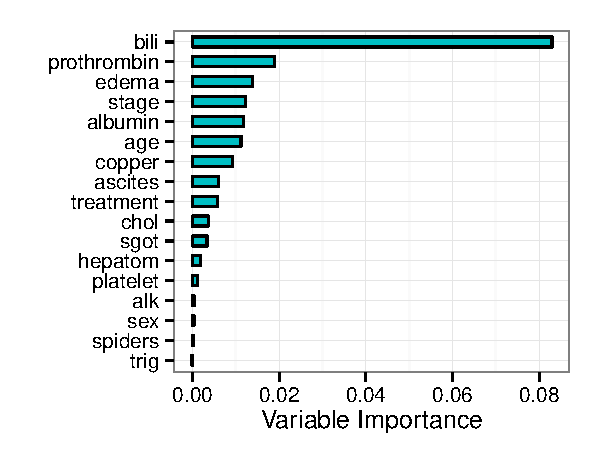
\includegraphics[width=\maxwidth]{figure/rfs-rf-vimp-1} 

}

\caption[Random forest variable Importance (VIMP)]{Random forest variable Importance (VIMP). Blue bars indicate important variables (positive VIMP), red indicates noise variables (negative VIMP).\label{fig:rf-vimp}}
\end{figure}
\end{Schunk}

\subsection{Minimal Depth}\label{S:minimalDepth}
In VIMP, prognostic risk factors are determined by inspection of the forest, ranking the most important variables according to impact on predictive ability of the forest. An alternative method recognizes that most important variables for prediction are those that most frequently split nodes nearest to the trunks of the trees (ie, at the root node) since they partition the largest portions of the population. 

Node levels are numbered based on their relative distance to the trunk of the tree (ie. 0, 1, 2). A measure of important risk factors is determined by averaging the depth of first split for each variable over all trees within the forest. Lower values of this measure indicate variables that split larger groups of patients. 

The maximal subtree for a variable $x$ is the largest subtree whose root node splits on $x$. Thus, all parent nodes of $x$'s maximal subtree have nodes that split on variables other than $x$. The largest maximal subtree possible is the root node. In general, however, there can be more than one maximal subtree for a variable. A maximal subtree may also not exist if there are no splits on the variable. The minimal depth of a maximal subtree (the first order depth) measures predictiveness of a variable $x$. It equals the shortest distance (the depth) from the root node to the parent node of the maximal subtree (zero is the smallest value possible). The smaller the minimal depth, the more impact $x$ has on prediction. The mean of the minimal depth distribution is used as the threshold value for deciding whether a variable's minimal depth value is small enough for the variable to be classified as strong. 

The minimal depth plot of Figure~\ref{fig:mindepth} is similar to the VIMP plot in Figure~\ref{fig:rf-vimp}, ranking variables from most important at the top (minimal depth measure), to least at the bottom (maximal minimal depth). Since the VIMP and Minimal Depth measures use different criteria, we expect the variable ranking to be slightly different. In this case, minimal depth indicates seven most important variables (op\_yr (surgical date), age, ld, ht, wt, iv\_lospr (length of stay) and inr). The vertical dashed line indicates the minimal depth threshold where smaller minimal depth values indicate higher importance and larger indicate lower importance.


\begin{Schunk}
\begin{Sinput}
R> varsel_pbc <- var.select(rfsrc_pbc)
R> ggMindepth <- gg_minimal_depth(varsel_pbc, lbls = st.labs)
R> print(ggMindepth)
\end{Sinput}
\end{Schunk}

\begin{Schunk}
\begin{Soutput}
-----------------------------------------------------------
gg_minimal_depth
model size         : 12 
depth threshold    : 5.5811 

PE :[1] 16.01
-----------------------------------------------------------

Top variables:
            depth  vimp
bili        1.724 0.068
albumin     2.535 0.014
copper      2.645 0.020
prothrombin 2.841 0.014
chol        3.245 0.005
age         3.466 0.009
edema       3.554 0.017
platelet    3.628 0.002
sgot        3.773 0.008
alk         3.947 0.000
trig        4.233 0.001
stage       4.546 0.009
-----------------------------------------------------------
\end{Soutput}
\end{Schunk}

\begin{Schunk}
\begin{Sinput}
R> plot(ggMindepth, lbls = st.labs)
\end{Sinput}
\begin{figure}[!htpb]

{\centering 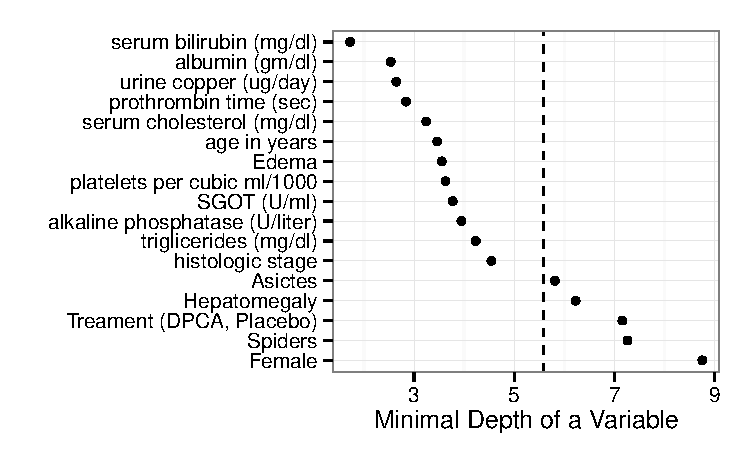
\includegraphics[width=\maxwidth]{figure/rfs-mindepth-plot-1} 

}

\caption[Minimal Depth variable selection]{Minimal Depth variable selection. Low minimal depth indicates important variables. The dashed line is the threshold of maximum value for variable selection.\label{fig:mindepth-plot}}
\end{figure}
\end{Schunk}

\begin{Schunk}
\begin{figure}[!htpb]

{\centering 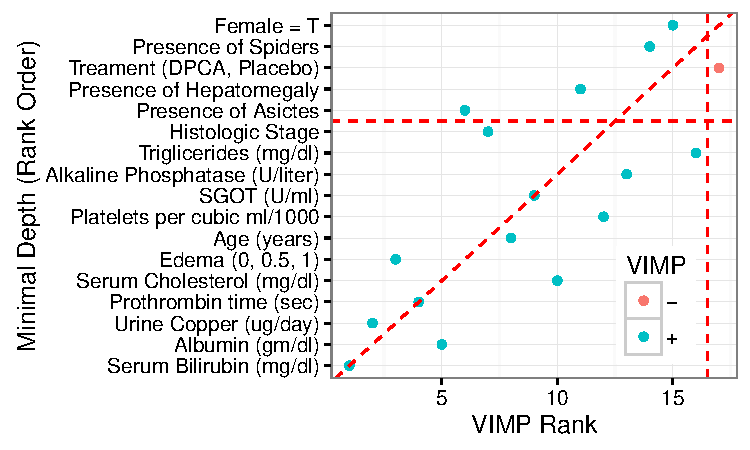
\includegraphics[width=\maxwidth]{figure/rfs-depthVimp-1} 

}

\caption[Comparing Minimal Depth and Vimp rankings]{Comparing Minimal Depth and Vimp rankings. Points on the red dashed line are ranked equivalently, points below have higher VIMP, those above have higher minimal depth ranking. Variables are colored by the sign of the VIMP measure.\label{fig:depthVimp}}
\end{figure}
\end{Schunk}

\section{Variable Dependence}\label{S:dependence}
Once we have an idea of which variables contribute to the predictive accuracy of the forest, it is useful to get some idea of form of this contribution. We use graphical methods to show the predicted response given dependence on covariates. We can plot the marginal effect of an covariate on the class probability (classification), response (regression), mortality (survival), or the expected years lost (competing risk) for a RF analysis. We plot the ensemble predicted value on the vertical axis and covariates along the horizontal axis.

\subsection{Marginal Dependence}\label{S:variableDependence}
\emph{Marginal variable dependence} plots the predicted response as a function of the covariate, showing each subject as a point on the plot. For classification and regression, this is straight forward predicting the response. In survival settings, we must account for the additional dimension of time. In this case, we plot the response at a specific time point of interest, for example survival at three months shown by the vertical dashed line in Figure~\ref{fig:rfsrc-plot3Mnth}. We take the predicted value of each curve at that time, and plot that against the covariate value for that observations, shown in Figure~\ref{fig:variable-plot}. Again censored cases are shown in blue circles, events are indicated by the red "x" symbols. Each predicted point is dependent on the full combination of all other covariates, not only on the covariate displayed in the dependence plot, so interpretation of these variable dependence plots can only be in general terms. The smooth loess line~\citep{cleveland:1981, cleveland:1988} indicates the trend of the prediction over surgical date progression.

\begin{Schunk}
\begin{Sinput}
R> ggRFsrc + 
+   geom_vline(aes(xintercept = c(1, 3)), linetype = "dashed") + 
+   coord_cartesian(x = c(0, 4))
\end{Sinput}
\begin{figure}[!htpb]

{\centering 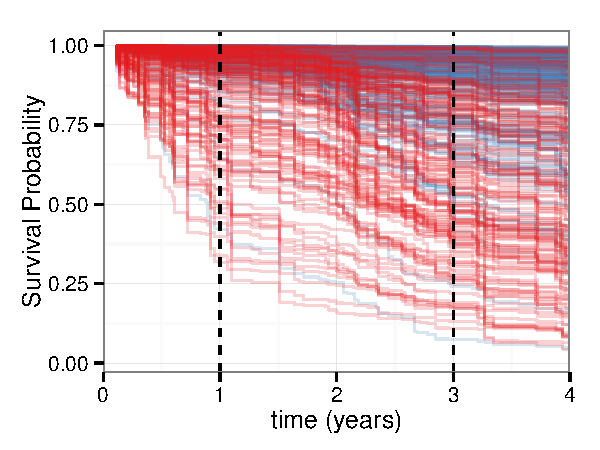
\includegraphics[width=\maxwidth]{figure/rfs-rfsrc-plot3Mnth-1} 

}

\caption[Random forest OOB predicted patient survival]{Random forest OOB predicted patient survival. Red curves correspond to patients which have died, blue corresponds to alive (or censored) cases. Vertical dashed lines indicate the 1 and 3 year survival estimates.\label{fig:rfsrc-plot3Mnth}}
\end{figure}
\end{Schunk}

\begin{Schunk}
\begin{Sinput}
R> xvar <- varsel_pbc$topvars[1:7]
R> 
R> ggrf <- gg_variable(rfsrc_pbc, time = c(1, 3), 
+                     time.labels = c("1 Year", "3 Years"))
R> 
R> plot(ggrf, xvar = xvar[1], se=.95, alpha=.3) + 
+   labs(y = "Survival") + 
+   theme(legend.position = "none") + 
+   scale_color_manual(values = strCol, labels = event.labels) + 
+   scale_shape_manual(values = event.marks, labels = event.labels)
\end{Sinput}
\begin{figure}[!htpb]

{\centering 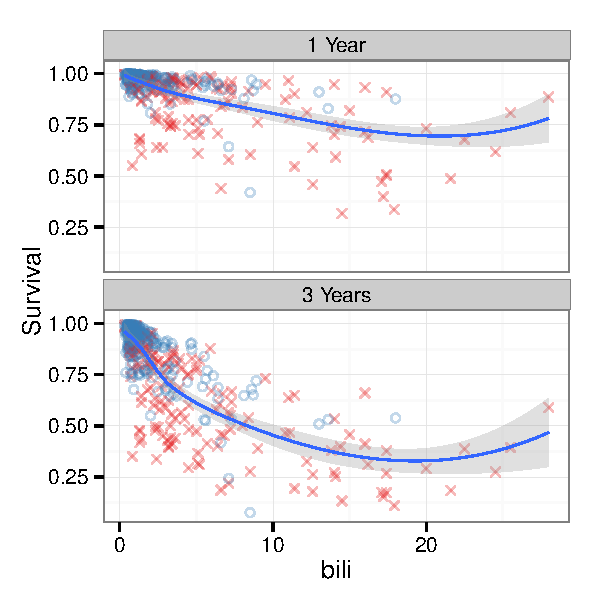
\includegraphics[width=\maxwidth]{figure/rfs-variable-plotbili-1} 

}

\caption[Bilirubin variable dependence at 1 and 3 years]{Bilirubin variable dependence at 1 and 3 years. Individual cases are marked with blue circles (alive or censored) and red xs (dead). Loess smooth curve with shaded 95\% confidence band indicates the survival trend with increasing bilirubin.\label{fig:variable-plotbili}}
\end{figure}
\end{Schunk}

\begin{Schunk}
\begin{Sinput}
R> plot(ggrf, xvar = xvar[-c(1,7)], panel = TRUE, 
+      se=FALSE, alpha=.3, 
+      method="glm", formula=y~poly(x,2)) + 
+   labs(y = "Survival") + 
+   theme(legend.position = "none") + 
+   scale_color_manual(values = strCol, labels = event.labels) + 
+   scale_shape_manual(values = event.marks, labels = event.labels)+
+   coord_cartesian(y=c(-.1,1.02))
\end{Sinput}
\begin{figure}[!htpb]

{\centering 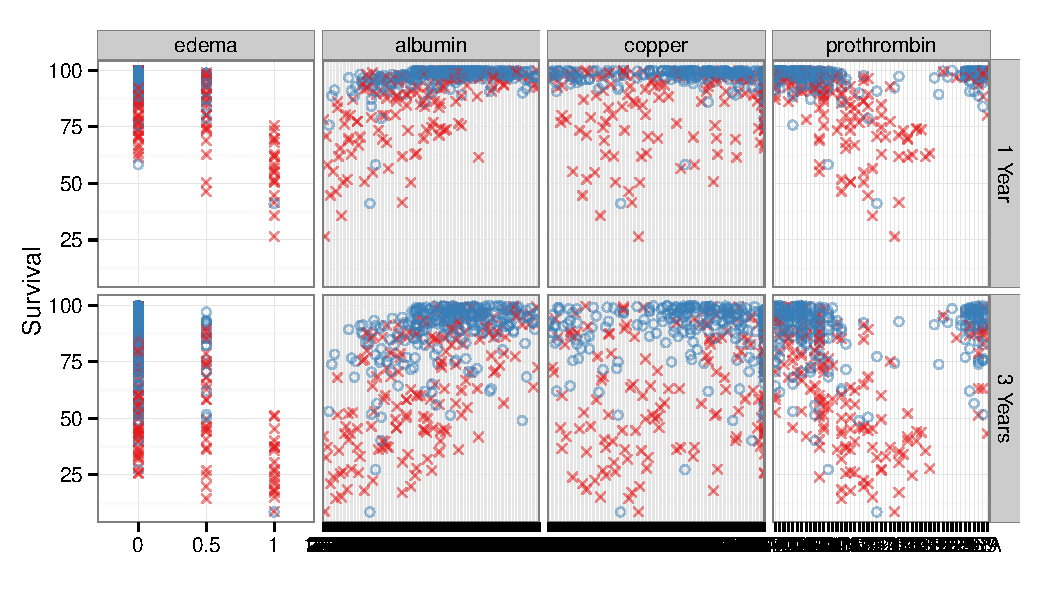
\includegraphics[width=\maxwidth]{figure/rfs-variable-plotCombines-1} 

}

\caption[Variable dependence plots at 1 and 3 years for continuous variables age, albumin, copper and prothrombin]{Variable dependence plots at 1 and 3 years for continuous variables age, albumin, copper and prothrombin. Individual cases are marked with blue circles (alive or censored) and red xs (dead). Loess smooth curve indicates the survival trend with increasing variable value.\label{fig:variable-plotCombines}}
\end{figure}
\end{Schunk}

\begin{Schunk}
\begin{Sinput}
R> plot(ggrf, xvar = "edema", notch=TRUE, alpha=.5) + 
+   labs(y = "Survival") + 
+   theme(legend.position = "none") + 
+   scale_color_manual(values = strCol, labels = event.labels) + 
+   scale_shape_manual(values = event.marks, labels = event.labels)+
+   coord_cartesian(y=c(-.1,1.02))
\end{Sinput}
\begin{figure}[!htpb]

{\centering \includegraphics[width=\maxwidth]{figure/rfs-variable-plotEdema-1} 

}

\caption[Variable dependence plots at 1 and 3 years for categorical edema variable]{Variable dependence plots at 1 and 3 years for categorical edema variable. Individual cases are marked with blue circles (alive or censored) and red xs (dead). Boxes indicate distributional properties of observations in each group.\label{fig:variable-plotEdema}}
\end{figure}
\end{Schunk}
\subsection{Partial Dependence}\label{S:partialDependence}

\emph{Partial dependence plots} are a risk adjusted alternative to marginal variable dependence. Partial plots are generated by integrating out the effects of variables beside the covariate of interest. The figures are constructed by selecting points evenly spaced along the distribution of the X variable. For each of these values (X = x), we calculate the average Random Forest prediction over all other covariates in X by \eqref{E:partial}.
\begin{equation}
\tilde{f}(x) = \frac{1}{n} \sum_{i = 1}^n \hat{f}(x, x_{i, o}), 
\label{E:partial}
\end{equation}
where $\hat{f}$ is the predicted response from the random forest and $x_{i, o}$ is the value for all other covariates other than $X = x$ for the observation $i$~\citep{Friedman:2000}. Partial dependence plots in time to event settings are shown at specific time points, similar to variable dependence.

Figure~\ref{fig:pbc-partial-bili} shows the partial dependence of three month survival on bilirubin. 

\begin{Schunk}
\begin{Sinput}
R> # Calculate the 1, 3 and 5 year partial dependence
R> partial_pbc <- lapply(c(1,3,5), function(tm){
+   plot.variable(rfsrc_pbc, surv.type = "surv", 
+                 time = tm, 
+                 xvar.names = xvar, partial = TRUE, 
+                 show.plots = FALSE)
+   })
\end{Sinput}
\end{Schunk}




\begin{Schunk}
\begin{Sinput}
R> # Convert all partial plots to gg_partial objects
R> gg_dta <- lapply(partial_pbc, gg_partial)
R> 
R> # Combine the objects to get multiple time curves 
R> # along variables on a single figure.
R> pbc_ggpart <- combine.gg_partial(gg_dta[[1]],gg_dta[[2]], 
+                                  lbls = c("1 Year", "3 Years"))
R> 
R> plot(pbc_ggpart[["bili"]], se = FALSE) + 
+   theme(legend.position = c(.8, .5)) + 
+   labs(y = "Survival", 
+        x = st.labs["bili"],
+        color="Time", shape="Time")+
+   scale_color_brewer(palette="Set1")
\end{Sinput}
\begin{figure}[!htpb]

{\centering 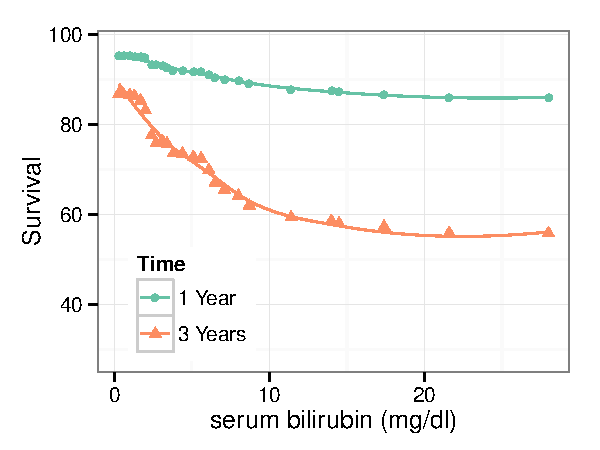
\includegraphics[width=\maxwidth]{figure/rfs-pbc-partial-bili-1} 

}

\caption[Partial dependence plot of (risk adjusted) predicted survival probability as a function of serum bilirubin at 1 year (red circle) and 3 years (blue triangle)]{Partial dependence plot of (risk adjusted) predicted survival probability as a function of serum bilirubin at 1 year (red circle) and 3 years (blue triangle). Loess smooth curves indicates the trend.\label{fig:pbc-partial-bili}}
\end{figure}
\end{Schunk}

Non-proportional hazards are evident in Figure~\ref{fig:pbc-partial-bili}.

\begin{Schunk}
\begin{Sinput}
R> # Create a temporary holder and remove the bilirubin and edema data
R> ggpart <- pbc_ggpart
R> ggpart$edema <- NULL
R> 
R> # Panel plot the remainder.
R> plot(ggpart, se = FALSE, panel = TRUE) + 
+   labs(x = "", y = "Survival",color="Time", shape="Time") +
+   scale_color_brewer(palette="Set1")
\end{Sinput}
\begin{figure}[!htpb]

{\centering 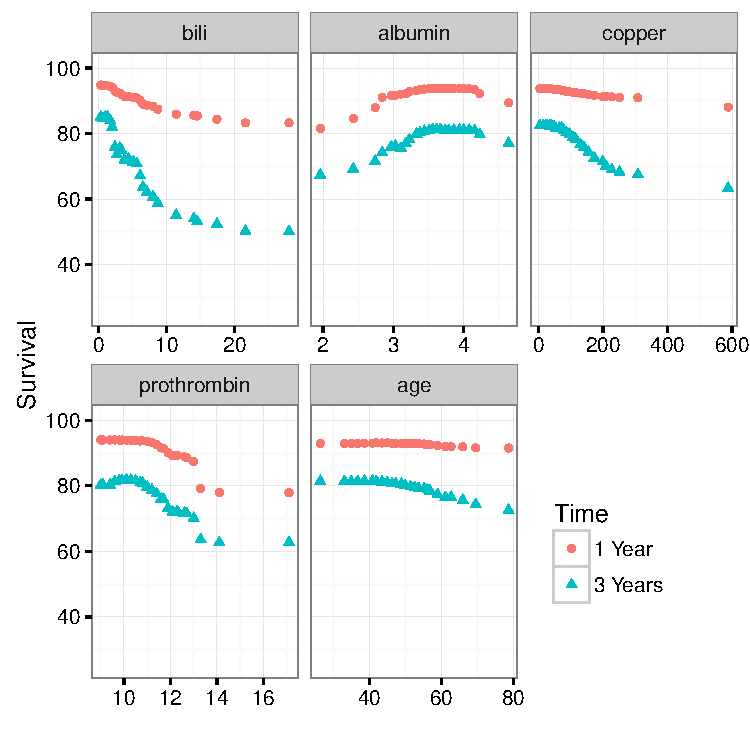
\includegraphics[width=\maxwidth]{figure/rfs-pbc-partial-panel-1} 

}

\caption[Partial dependence plot of (risk adjusted) predicted survival probability as a function continuous variables prothrombin time, albumin, age and urin copper at 1 year (red circle) and 3 years (blue triangle)]{Partial dependence plot of (risk adjusted) predicted survival probability as a function continuous variables prothrombin time, albumin, age and urin copper at 1 year (red circle) and 3 years (blue triangle).\label{fig:pbc-partial-panel}}
\end{figure}
\end{Schunk}

\begin{Schunk}
\begin{Sinput}
R> plot(pbc_ggpart$edema, notch=TRUE, alpha=.3, outlier.shape = NA) + 
+   labs(x = "Edema", y = "Survival (%)")+
+   scale_color_brewer(palette="Set1")+
+   facet_grid(~group)+
+   theme(legend.position="none")
\end{Sinput}
\end{Schunk}

\section{Variable Interactions}\label{S:interactions}
Using the different variable dependence measures, we can calculate pairwise interactions for any pair of variables. Minimal depth is calculated as the maximal subtree using the normalized minimal depth of variable $i$ relative to the root node (normalized with respect to the size of the tree). For interactions, we calculate the maximal subtree interaction measure as the normalized minimal depth of a variable $j$ with respect to the maximal subtree for variable $i$ (normalized with respect to the size of $i$'s maximal subtree)~\citep{Ishwaran:2010,Ishwaran:2011}.

\begin{Schunk}
\begin{Sinput}
R> interaction_pbc <- find.interaction(rfsrc_pbc)
R> 
R> ggint <- gg_interaction(interaction_pbc)
R> plot(ggint, xvar = "bili") + 
+   labs(y = "Interactive Minimal Depth")
\end{Sinput}
\end{Schunk}

\begin{Schunk}
\begin{figure}[!htpb]

{\centering 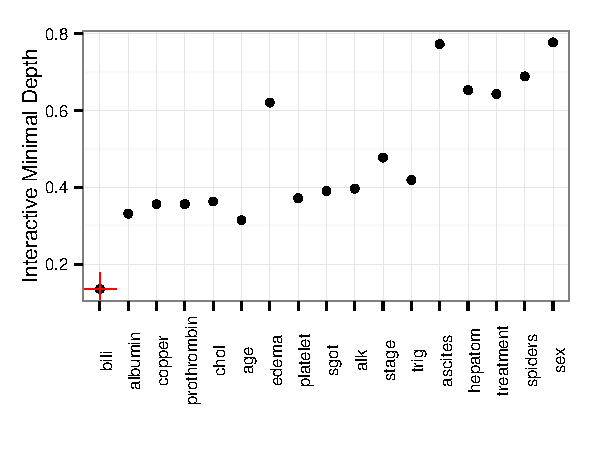
\includegraphics[width=\maxwidth]{figure/rfs-interaction-1} 

}

\caption[Minimal depth variable interaction with bilirubin (marked with red cross)]{Minimal depth variable interaction with bilirubin (marked with red cross). Higher values indicate lower interactivity with target variable.\label{fig:interaction}}
\end{figure}
\end{Schunk}

Measuring interactions with minimal depth results a $p \times p$ matrix of interaction measures, with smaller diagonal measures relative to the root node, and off diagonal measures of pairwise interaction. We expect the covariate with smallest minimal depth to have the highest interactive depth measures, so viewed alone may not be as informative as looking at other interactive depth plots. Figure~\ref{fig:interactionPanel} combines the remaining top ranked minimal depth measures for comparison.
\begin{Schunk}
\begin{Sinput}
R> plot(gg_interaction(interaction_pbc), xvar = xvar[-1]) + 
+   labs(y = "Interactive Minimal Depth") + 
+   theme(legend.position = "none")
\end{Sinput}
\begin{figure}[!htpb]

{\centering 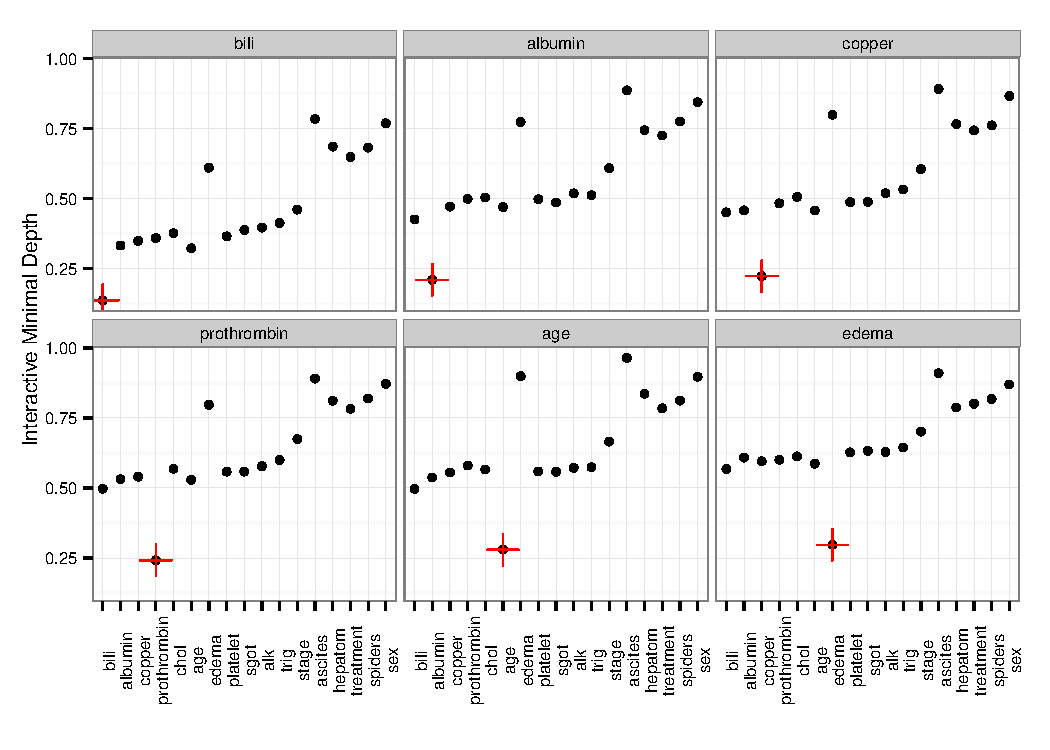
\includegraphics[width=\maxwidth]{figure/rfs-interactionPanel-1} 

}

\caption[Minimal depth variable interaction panel with prothrombin time, albumin, urine copper and edema]{Minimal depth variable interaction panel with prothrombin time, albumin, urine copper and edema. Higher values indicate lower interactivity with target variable.\label{fig:interactionPanel}}
\end{figure}
\end{Schunk}

\subsection{Conditional Dependence Plots}

By plotting the resulting interaction measures for each variable (Figure~\ref{fig:interaction}), we can detect the "most interactive" pairs, and develop conditional plots~\cite{chambers:1992, cleveland:1993}. These plots are similar to stratified results, arranged in a set of panels by the interactive variable of interest. 

Interactions with categorical data are more straight forward, and can be generated directly from variable dependence plots. Recall the 1 year variable dependence for Billirubin, shown in Figure~\ref{fig:var_dep}. 
\begin{Schunk}
\begin{Sinput}
R> ggvar <- gg_variable(rfsrc_pbc, time = 1)
R> ggvar$stage <- paste("stage=", ggvar$stage, sep="")
R> 
R> var_dep <- plot(ggvar, xvar = "bili", smooth = TRUE, 
+                 method = "loess", span=1.5,alpha = .5, se = FALSE) + 
+   labs(y = "Survival", 
+        x = st.labs["bili"]) + 
+   theme(legend.position = "none") + 
+   scale_color_manual(values = strCol, labels = event.labels) + 
+   scale_shape_manual(values = event.marks, labels = event.labels)
R> 
R> show(var_dep)
\end{Sinput}
\begin{figure}[!htpb]

{\centering 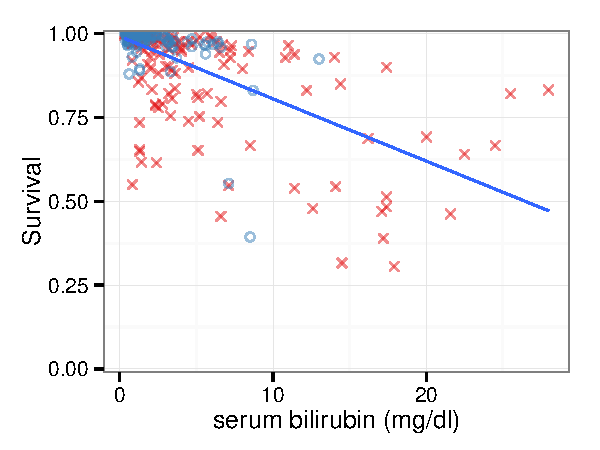
\includegraphics[width=\maxwidth]{figure/rfs-var_dep-1} 

}

\caption[Variable dependence plot]{Variable dependence plot. Survival at 1 year against bilirubin. Individual cases are marked with blue circles (alive or censored) and red x (dead). Loess smooth curve indicates the trend as bilirubin  increases.\label{fig:var_dep}}
\end{figure}
\end{Schunk}

We can view the conditional dependence of survival against bilirubin, versus other categorical covariates, say treatment (binary) and stage (categorical), by adding a facet argument.
\begin{Schunk}
\begin{Sinput}
R> var_dep + 
+   facet_grid(treatment~stage)
\end{Sinput}
\begin{figure}[!htpb]

{\centering 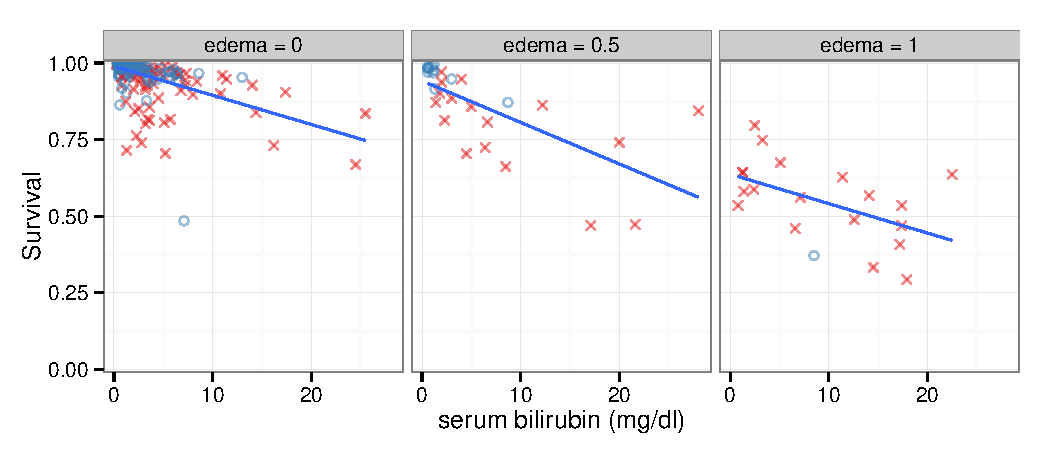
\includegraphics[width=\maxwidth]{figure/rfs-coplot_bilirubin-1} 

}

\caption[Variable dependence coplot]{Variable dependence coplot. Survival at 1 year against bilirubin, stratified by treatment and histological stage.\label{fig:coplot_bilirubin}}
\end{figure}
\end{Schunk}

Interactions with continuous variables requires stratification at some level.

\subsection{Albumin}
\begin{Schunk}
\begin{Sinput}
R> # albumin_grp <- cut(rfsrc_pbc$xvar$albumin, breaks=c(0,seq(3,3.5,.5),5))
R> albumin_grp <- cut(rfsrc_pbc$xvar$albumin, breaks=6)
R> ggvar$albumin_grp <- paste("albumin=",albumin_grp, sep="")
R> 
R> var_dep <- plot(ggvar, xvar = "bili", smooth = TRUE, 
+                 method = "loess", span=1.5,alpha = .5, se = FALSE) + 
+   labs(y = "Survival", x = st.labs["bili"]) + 
+   theme(legend.position = "none") + 
+   scale_color_manual(values = strCol, labels = event.labels) + 
+   scale_shape_manual(values = event.marks, labels = event.labels)+ 
+   facet_wrap(~albumin_grp)
R> 
R> var_dep
\end{Sinput}
\begin{figure}[!htpb]

{\centering 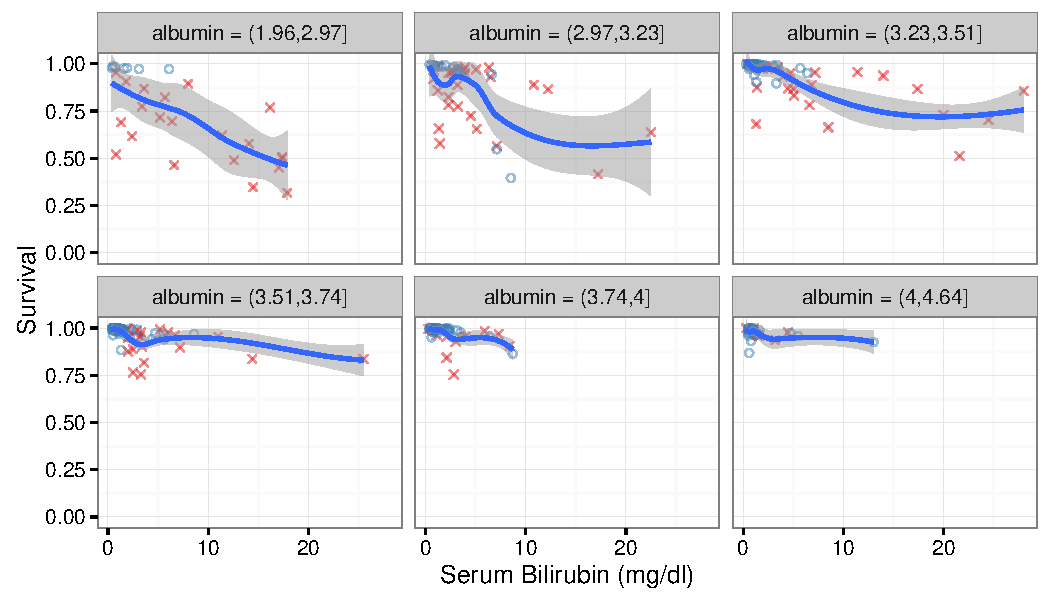
\includegraphics[width=\maxwidth]{figure/rfs-albumin-coplot-1} 

}

\caption[Variable dependence coplot]{Variable dependence coplot. Survival at 1 year against bilirubin, stratified by continous variable albumin.\label{fig:albumin-coplot}}
\end{figure}
\end{Schunk}



\begin{Schunk}
\begin{Sinput}
R> data(partial_coplot_pbc, package="ggRandomForests")
R> ggpl <- ggplot(partial_coplot_pbc, aes(x=bili, y=yhat, 
+                                           shape=group, 
+                                           color=group))+
+   geom_point()+geom_smooth(se=FALSE)+
+   labs(x=st.labs["bili"], y="Survival 1 year", 
+        color="Albumin", shape="Albumin")+
+   scale_color_brewer(palette="Set1")
R> ggpl
\end{Sinput}
\begin{figure}[!htpb]

{\centering 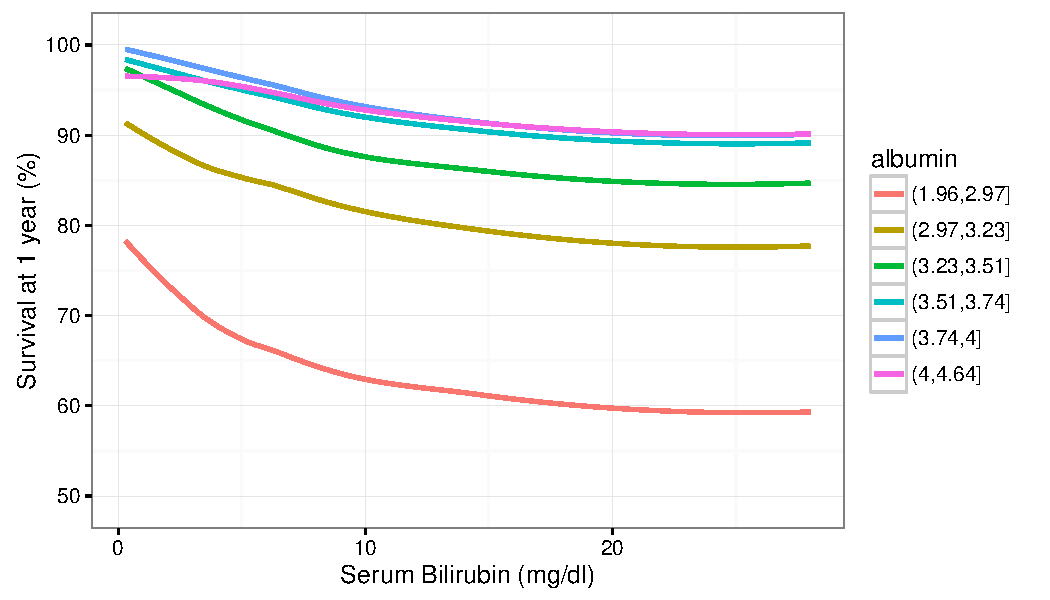
\includegraphics[width=\maxwidth]{figure/rfs-bili-albumin-1} 

}

\caption[Partial (risk adjusted) variable dependence coplot]{Partial (risk adjusted) variable dependence coplot. Survival at 1 year against bilirubin, stratified by albumin groups. Points mark risk adjusted estimates, loess smooth indicates predicted trend within each age group as a function of bilirubin.\label{fig:bili-albumin}}
\end{figure}
\end{Schunk}

\section{Conclusion}

\appendix

%\singlespacing
\bibliography{ggRandomForests}

\end{document}
